\section{Complexity Analysis via Symbolic Execution Schemes}
\label{sec:symbolic}

Our approach to complexity analysis is based on a semi-automatic procedure involving symbolic evaluation.
In the previous section we presented formulae to compositionally estimate the complexity factors for
\emph{non-leaf states} of operational semantics under assumption that coresponding estimations for
\emph{leaf states} are given. In order to obtain corresponding estimations for relations we
would need to take into account the effects of relational invocations, including the recursive ones.

Another observation is that as a rule we are interested in complexity estimations in terms of some \emph{metatheory}. For
example, dealing with relations on lists we would be interested in estimations in terms of list lengths,
with trees~--- in terms of depth or number of nodes, with numbers~--- in terms of their values, etc. It is
unlikely that a generic term-based framework would provide such a specific information automatically. Thus,
a viable approach would be to extract some inequalities involving the complexity factors of certain relational
calls automatically and then let a human being solve these inequalities in terms of a relevant metatheory.

For clarity we will provide demonstration of the complexity analysis for a specific example -- \lstinline|append$^o_{naive}$| relation from the introduction  -- throughout the section.

The extraction procedure utilizes the symbolic execution technique and is completely automatic.
It turns out that the semantics we have is already abstract enough to be used for symblolic
execution with minor adjustments.
In this symbolic procedure we mark some of the logic variables as ``grounded'' and at certain
moments substitute them with ground terms.
Informally, for some goal with some free logic variables we consider the complexity of a search
procedure which finds the bindings for all non-grounded variables based on the ground values
substituted for the grounded ones.
This seach procedure is defined precisely by the operational semantics; however, as the concrete
values of grounded variables are unknown (only the fact of their \emph{groundness}), the whole
procedure becomes symbolic.
In particular, in unification the groundness can be propagated to some non-grounded free variables.
Thus, the symbolic execution is determined by the subset of grounded varibles (hereafter denoted
as $V\subset\mathcal A$).
The initial choice of $V$ defines the problem we analyze.

For our example, we want to study the execution when we specialize the first two arguments with
ground values and left the last argument with free variable. 
So we start with the goal \lstinline|append$^o_{naive}$ $a$ $b$ $ab$| (with three distinct logic variables
$a$, $b$ and $ab$) and set the initial $V = \{ a, b \}$.

It is important to note that both our complexity factors are stable w.r.t. renaming of free
variables.
The measures are also stable w.r.t. change of the fresh variables counter, as long as it stays
adequate, and change of current substitution, as long as it gives the same terms after application.
This observation shows that it does not matter at which point of execution a relational call is invoked and so
we can analyze every call separatelly.

\begin{replemma}{lem:measures_changing_env}

Let $s = \taskst{g}{\mkenv{\sigma}{n}}$ and $s' = \taskst{g^\prime}{\mkenv{\sigma^\prime}{n^\prime}}$ be two well-formed states.
If  there exists a bijective substitution $\pi \colon FV\,(g \sigma) \to FV\,(g^\prime \sigma^\prime)$  such that  $g \sigma \pi = g^\prime \sigma^\prime $, then $d\,(s) = d\,(s^\prime)$ and $t\,(s) = t\,(s^\prime)$.
\end{replemma}

We therefore can construct an initial state for any given goal using the following definition and
analyze its execution.

\begin{definition} Let $g$ be a goal. An initial state for $g$ is $init\,(g)=\taskst{g}{(\varepsilon, \ninit\,(g))} $ with $ n_{init}\,(g) = \min\, \{ n \mid FV\,(g) \subseteq \{ \alpha_1\dots\alpha_n \} \} $
\end{definition}

For our example, we will be studying the family of initial states $q^{appn}(\mathbf{a}, \mathbf{b}) = init\,(\lstinline|append$^o_{naive}$ $\mathbf{a}$ $\mathbf{b}$ $ab$|)$ with arbitrary ground terms $\mathbf{a}$ and $\mathbf{b}$.

We are aiming at the complexity function depending on specific ground values substituted for grounded variables, so in general case extracted inequalities will be parameterized by \emph{valuations}~--- mappings from the set of grounded variables to ground terms. As the new variables are added to this set during execution, the valuations need to be extended on these new variables. We will use the following definition to capture it.

\begin{definition}
  Let $ V \subset U \subset \mathcal{A} $ and $ \rho \colon V \to \mathcal{T}_{\emptyset} $ and $ \rho^\prime \colon U \to \mathcal{T}_{\emptyset} $ be two valuations. We say that $\rho^\prime$ extends $\rho$ (denotation: $ \rho^\prime \succ \rho$) if $\rho^\prime\,(x) = \rho\,(x)$ for all $x \in V$.
\end{definition}

The main objective of the symbolic execution in our case is to find constraints on valuations for every basic goal in the body of a relation that determine whether the execution will continue and how valuation change after this goal.

For internal relational calls we will describe constraints in term of denotational semantics (to be later given meaning inside metatheory). We can do it beacuse of precise equivalence between the anwers found by operational semantics and values described by denotational semantics thanks to soundness and completness as well as our requirements of grounding and non-repetitiveness of calls.

Our symbolic treatment of equalities will rely on the fact that subtitution of ground terms commutes, in a certain sense, with unification. More specifically, we can use the most general unifier for two terms to see how unification goes for these two terms with some free variables substituted with ground terms. The most general unifier may contain bindings for both grounded and non-grounded variables. Potential most general unifier for terms after substitution contains the same bindings for non-grounding terms (with valuation applied to their rhs), while bindings for grounding variables turn into equations that should be satisfied by unifier with ground value on the left and binded term on the right. In particular, this means that all variables in bindings for grounded variables become grounded too. We can use this observation to define an iterative process that determines the updated set of grounded variables $\upd{U}{\delta}$ for a current set $U$ and a most general unifier $\delta$ and a set of equations $\constr{\delta}{U}$ that should be satisfied by the valuation.

\[
\upd{U}{\delta} = \begin{cases}
                           U & \quad\forall x \in U : FV\,(\delta\,(x)) \subset U \\
                           \upd{U \cup \displaystyle\bigcup\limits_{x \in U} FV\,(\delta\,(x))}{\delta} & \quad\mbox{otherwise}
                          \end{cases}
\]

\[ \constr{\delta}{U} = \{ x = \delta\,(x) \mid x \in U \cap \mathcal{D}om\,(\delta) \} \]

Using these definitions we can describe symbolic unification in our case by the following lemma.

\begin{replemma}{lem:symbolic_unification_soundness}
Let $t_1$, $t_2$ be terms,  $V \subset \mathcal{A}$ and $\rho \colon V \to \grterms$ be a valuation. If $mgu\,(t_1, t_2) = \delta$ and $U = \upd{V}{\delta} $  then $t_1 \rho$ and $t_2 \rho$ are unifiable iff there is some $\rho' \colon U \to \grterms$ such that $\rho' \succ \rho$ and $\forall (y = t) \in \constr{\delta}{U}\,:\, t_1 \rho = t_2 \rho'$.
In such case $\rho'$ is unique and $ \rho \circ mgu\,(t_1 \rho, t_2 \rho) = \delta\circ\rho' $ up to alpha-equivalence (e.g. there exists a bijective substitution $\pi : FV(t_1) \to FV(t_2)$, s.t. $ \rho \circ mgu\,(t_1 \rho, t_2 \rho) = \delta \circ\rho'\circ \pi$).
\end{replemma}

Our extraction will be based on a visual representation of execution of the body of a relation for a given set of grounded variables as a symbolic scheme. It is a tree structure with differenct branches corresponding to different disjuncts and nodes that are internal equalities and relational calls in the body, with specified subset of variables that are grounded at the point of their execution.~\footnote{Notice that the difference with usual symbolic execution graphs with different branches representing mutually exclusive possible paths of evaluation, not the different parts of one evaluation.} Constrains on substituted grounded variables that determine whether the execution continues are presented as labels on edges of a scheme.

More formally, each scheme has one of the following 5 forms (scheme is indexed by the subset of grounded variables, $\Upsilon = 2^{\mathcal{A}}$ denoting such subsets).

\[
\renewcommand{\arraystretch}{3}
\begin{array}{ccm{0.5cm}m{3cm}m{4cm}m{4cm}}
  \schemewithvset{\mathfrak{S}}{\Upsilon} & = && \schemenode{$\unigoal{\mathcal{T}_\mathcal{A}}{\mathcal{T}_\mathcal{A}}$} & \schemenode{$\invokegoal{R^k}{\mathcal{T}_\mathcal{A}}{\mathcal{T}_\mathcal{A}}$} 
                                       & \multirow{2}{*}{\schemefork{$\schemewithvset{\mathfrak{S}}{\Upsilon}$}{$\schemewithvset{\mathfrak{S}}{\Upsilon}$}} \\
                                   &   && \schemesarrow{$\unigoal{\mathcal{T}_\mathcal{A}}{\mathcal{T}_\mathcal{A}}$}{$\{\mathcal{A}=\mathcal{T}_\mathcal{A}\}$}{$\schemewithvset{\mathfrak{S}}{\Upsilon}$}
                                       & \schemedarrow{$\invokegoal{R^k}{\mathcal{T}_\mathcal{A}}{\mathcal{T}_\mathcal{A}}$}{$(\mathcal{T}_\mathcal{A}, \dots, \mathcal{T}_\mathcal{A}) \in \sembr{R^k}$}{$\schemewithvset{\mathfrak{S}}{\Upsilon}$}
                                       & 
\end{array}
\]

Notice that constrains after nodes of different types differ: unification puts a constraint in form of set of equations on substituted ground values that should be satisfied and relational call puts a constraint in form of a tuple of ground terms that should belong to denotational semantics of a relation.

Construction of a scheme for the given goal (initially, the body of a relation) mimics ordinary execution of a relational program. The deriavtion rules for scheme formation have the following form.
\[ \schemetrans{g}{\Gamma}{\sigma}{n}{V}{\schemewithvset{\mathfrak{S}}{V}} \]
Here $g$ is the given goal, $\Gamma$ is the list of postponed goals (these goals should be executed after the execution of $g$ in every branch in the same order, initially this list is empty), $\sigma$ and $n$ are the substitution and the counter from the current substitution respectively, $V$ is a set of grounded variables at the moment.

\begin{figure}[t]  
\renewcommand{\arraystretch}{3}
  \[
\begin{array}{cr}
  \onepremrule
		{  \schemetrans{g_1}{g_2 : \Gamma}{\sigma}{n}{V}{\schemewithvset{\mathfrak{S}}{V}}  } 
		{  \schemetrans{\conjgoal{g_1}{g_2}}{\Gamma}{\sigma}{n}{V}{ \schemewithvset{\mathfrak{S}}{V} }  } & \ruleno{Conj$_\mathfrak S$}
		\\
                
  % \multicolumn{3}{c}{
  \twopremrule
		{  \schemetrans{g_1}{\Gamma}{\sigma}{n}{V}{\schemewithvset{\mathfrak{S_1}}{V}}  }
		{  \schemetrans{g_2}{\Gamma}{\sigma}{n}{V}{\schemewithvset{\mathfrak{S_2}}{V}}  }
		{  \schemetrans{\disjgoal{g_1}{g_2}}{\Gamma}{\sigma}{n}{V}{\parbox[m]{2cm}{ \schemefork{$\schemewithvset{\mathfrak{S_1}}{V}$}{$\schemewithvset{\mathfrak{S_2}}{V}$}} }  } & \ruleno{Disj$_\mathfrak S$}\\ 
		
		
 \onepremrule
		{  \schemetrans{\substitute{g}{\alpha_n}{x}}{\Gamma}{\sigma}{n + 1}{V}{\schemewithvset{\mathfrak{S}}{V}}  }
		{  \schemetrans{\freshgoal{x}{g}}{\Gamma}{\sigma}{n}{V}{ \schemewithvset{\mathfrak{S}}{V} }  } & \ruleno{Fresh$_\mathfrak S$}\\

 %\multicolumn{3}{c}{
  \schemetrans{\unigoal{t_1}{t_2}}{\epsilon}{\sigma}{n}{V}{\parbox[m]{2cm}{\schemenode{$\unigoal{t_1 \sigma}{t_2 \sigma}$}}}& \ruleno{UnifyLeaf$_\mathfrak S$}\\

 %\multicolumn{3}{c}{
 \schemetrans{\invokegoal{R^k}{t_1}{t_k}}{\epsilon}{\sigma}{n}{V}{\parbox[m]{2cm}{\schemenode{$\invokegoal{R^k}{t_1 \sigma}{t_k \sigma}$}}}& \ruleno{InvokeLeaf$_\mathfrak S$}\\ 
		
 %\multicolumn{3}{c}{
  \onepremrule
		{  \nexists mgu\,(t_1 \sigma, t_2 \sigma)  }
		{  \schemetrans{\unigoal{t_1}{t_2}}{g : \Gamma}{\sigma}{n}{V}{\parbox[m]{2cm}{\schemenode{$\unigoal{t_1 \sigma}{t_2 \sigma}$}}} }& \ruleno{UnifyFail$_\mathfrak S$}\\

 %\multicolumn{3}{c}{
  \threepremrule
		{  mgu\,(t_1 \sigma, t_2 \sigma) = \delta  }
		{  U = \upd{V}{\delta}  }
		{  \schemetrans{g}{\Gamma}{\sigma \delta}{n}{U}{\schemewithvset{\mathfrak{S}}{U}}  }
		{  \schemetrans{\unigoal{t_1}{t_2}}{g : \Gamma}{\sigma}{n}{V}{\parbox[m]{2cm}{\schemesarrow{$\unigoal{t_1 \sigma}{t_2 \sigma}$}{$\constr{\delta}{U}$}{$\schemewithvset{\mathfrak{S}}{U}$}} }   } & \ruleno{UnifySuccess$_\mathfrak S$}\\
		
 %\multicolumn{3}{c}{
  \twopremrule
		{  \mbox{\phantom{XXXXXX}} U =  V \cup \displaystyle\bigcup\limits_{i} FV\,(t_i \sigma) }
		{  \schemetrans{g}{\Gamma}{\sigma}{n}{U}{\schemewithvset{\mathfrak{S}}{U}} \mbox{\phantom{XXXXXX}} }
		{  \schemetrans{\invokegoal{R^k}{t_1}{t_k}}{g : \Gamma}{\sigma}{n}{V}{ \parbox[m]{2cm}{\schemedarrow{$\invokegoal{R^k}{t_1 \sigma}{t_k \sigma}$}{$ (t_1 \sigma, \dots, t_k \sigma) \in \sembr{R^k} $}{$\schemewithvset{\mathfrak{S}}{U}$}} }   } & \ruleno{Invoke$_\mathfrak S$}
 \end{array}
\]
\caption{Scheme Formation Rules}
\label{fig:scheme_formation}
\end{figure}

The rules are shown on \figureword~\ref{fig:scheme_formation}. \ruleno{Conj$_\mathfrak S$} and \ruleno{Disj$_\mathfrak S$} are structural rules: when investigatig conjunctions we postpone the second conjuct by putting it in the list $\Gamma$ and continue with the first conjunct, disjunctions we simply present as forks. \ruleno{Fresh$_\mathfrak S$} introduses a fresh logic variable (not grounded) and updates counter of occupied variables accordingly. When investigated goal is equality or relational call it is added as node to the scheme. If there are no postponed goals, it is just added as a leaf (rules \ruleno{UnifyLeaf$_\mathfrak S$} and \ruleno{InvokeLeaf$_\mathfrak S$}). Equality is also added as a leaf if there are postponed goals, but the terms are non-unifiable and so the execution stops (rule \ruleno{UnifyFail$_\mathfrak S$}). If the terms in the equality are unifiable and there are postponed goals (rule \ruleno{UnifySuccess$_\mathfrak S$}), the equality is added as a node and the execution continues for postponed goals, starting with the fist one, and also the set of grounded variables is updated and constrains are added on the edge in accordance with \lemmaword~\ref{lem:symbolic_unification_soundness}. The same way for relational call if there are postponed goals (rule \ruleno{Invoke$_\mathfrak S$}), all variables occuring in the call become grounded (its the grounding condition we impose) and should satisfy the denotational semantics of the invoked relation.

\begin{figure}[t]
\begin{center}
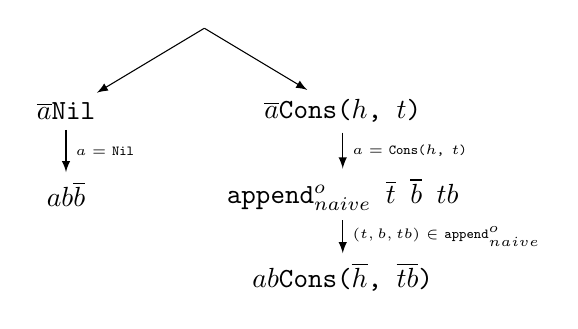
\begin{tikzpicture}[level distance=30pt, sibling distance=10em, edge from parent/.style={draw,-latex}]
   \coordinate   
      child { node {$\unigoal{\overline{a}}{\texttt{Nil}}$}
        child { node {$\unigoal{ab}{\overline{b}}$}
                  edge from parent node[right]{\tiny{${a} = \texttt{Nil}$}} } }
      child { node {$\unigoal{\overline{a}}{\texttt{Cons($h$, $t$)}}$} 
      	child { node {\texttt{append$^o_{naive}$ $\overline{t}$ $\overline{b}$ $tb$}}
      	   child { node {$\unigoal{ab}{\texttt{Cons($\overline{h}$, $\overline{tb}$)}}$}
      	             edge from parent node[right]{\tiny{$({t}, {b}, {tb}) \in \llbracket \texttt{append$^o_{naive}$} \rrbracket$}}  }
      	   edge from parent node[right]{\tiny{${a} = \texttt{Cons(${h}$, ${t}$)}$}}  } } ;
\end{tikzpicture}
\end{center}

\caption{Symbolic execution scheme for the goal  \lstinline|append$^o_{naive}$ $a$ $b$ $ab$|  with initial set of grounded variables $V = \{ a, b \}$. For each node, variables that are grounded at the point of execution of this node are overlined. }
\label{fig:example_scheme}
\end{figure}

The scheme constructed by these rules for our \lstinline|append$^o$| example is shown in \figureword~\ref{fig:example_scheme}. For simplicity we do not put the set of grounded variables for each node, but instead overline variables that are grounded. Note that all variables that occur in constraints on edges are grounded after the parent node is executed.

Now, we can use schemes to see how the basic goals in relation body are combined with conjunctions and disjuntions. Then we can apply formulae from \sectionword~\ref{sec:scheduling} to get recursive inequalities (providing lower and upper bounds simultaniously) for both complexity measures.

\begin{figure}[t]
\[
\begin{array}{rclcl}
 \mathcal{\nicefrac{D}{T}}\,(&\parbox[m]{1.3cm}{\schemenode{$\unigoal{t_2}{t_2}$}}&)(\rho) &=& 1  \\

 \mathcal{\nicefrac{D}{T}}\,(&\parbox[m]{2.5cm}{\schemenode{$\invokegoal{R^k}{t_1}{t_k}$}}&)(\rho) &=& \nicefrac{d}{t}\,(init\,(\invokegoal{R^k}{t_1 \rho}{t_k \rho})) \\

 \mathcal{\nicefrac{D}{T}}\,(&\parbox[m]{2cm}{\schemesarrow{$\unigoal{t_1}{t_2}$}{$Cs$}{$\schemewithvset{\mathfrak{S}}{U}$}} &)(\rho) &=& 1 +
      \sum\limits_{\substack{ \rho' \colon V \to \grterms \\
                                      \rho' \succ \rho \\
                                      \forall (y, t) \in Cs\,:\, \rho'\,(y) = t\, \rho'  }}
           \mathcal{\nicefrac{D}{T}}\,(\schemewithvset{\mathfrak{S}}{U})(\rho')  \\

 \mathcal{\nicefrac{D}{T}}\,(& \parbox[m]{4cm}{\schemedarrow{$\invokegoal{R^k}{t_1}{t_k}$}{ $(t_1, \dots, t_k) \in \sembr{R^k}  $}{$\schemewithvset{\mathfrak{S}}{U}$}} &)(\rho) &=&
      \nicefrac{d}{t}\,(init\,(\invokegoal{R^k}{t_1 \rho}{t_k \rho})) +
      \sum\limits_{\substack{ \rho' \colon V \to \grterms \\
                                      \rho' \succ \rho \\
                                      (t_1 \rho', \dots, t_k \rho') \in \sembr{R^k}  }}
           \mathcal{\nicefrac{D}{T}}\,(\schemewithvset{\mathfrak{S}}{U})(\rho')  \\

 \mathcal{\nicefrac{D}{T}}\,(&\parbox[m]{2.5cm}{\schemefork{$\schemewithvset{\mathfrak{S}_1}{V}$}{$\schemewithvset{\mathfrak{S}_2}{V}$}}&)(\rho) &=&
 \mathcal{\nicefrac{D}{T}}\,(\schemewithvset{\mathfrak{S}_1}{V})(\rho) + \mathcal{\nicefrac{D}{T}}\,(\schemewithvset{\mathfrak{S}_2}{V})(\rho)
\end{array}
\]
\caption{Complexity Measures Extraction: $\mathcal D$ and $\mathcal T$}
\label{fig:scheduling_extraction_d_t}
\end{figure}

In this inequalities we need to sum values of $d$-measure and $t$-measure for all basic goals of a body and for all environments that these basic goals are evaluated on. The basic goals are the nodes of a scheme and evaluated environments can be derived from constraints written on edges. So, for this summation we introduce the following notions: $\mathcal{D}$ is sum of $d$-measure values and $\mathcal{T}$ is sum of $t$-measure values for execution of the body with specific valuation $\rho$. Their defintions are shown in the \figureword~\ref{fig:scheduling_extraction_d_t} (they are written jointly, as these defintions coincide, only the measure changes). For nodes we take corresponding value (for equality it always equals to $1$). When going through an equality we sum the rest with updated valuation (by \lemmaword~\ref{lem:symbolic_unification_soundness} this sum always has one or zero summands depending on whether unification is successful or not). When going through a relational call we take a sum of all valuations that satisfy denotational semantics (these valuations will correspond exactly to the set of all answers produced by the call because operational semantics is sound and complete w.r.t. the denotational one and because we require all calls to be non-repetitive). For disjunctions we take sum of both branches.


\begin{figure}[t]
\colorbox{yellow!20}{\parbox{\textwidth}{\textbf{Maybe move this to appendix and leave here the informal description only}}}

\[
\begin{array}{rclcl}
 \mathcal{L}\,(&\parbox[m]{1.3cm}{\schemenode{$\unigoal{t_2}{t_2}$}}&)(\rho) &=& \{init\,(\unigoal{t_2}{t_2})\} \\

 \mathcal{L}\,(&\parbox[m]{2.5cm}{\schemenode{$\invokegoal{R^k}{t_1}{t_k}$}}&)(\rho) &=& \{init\,(\invokegoal{R^k}{t_1 \rho}{t_k \rho})\} \\

 \mathcal{L}\,(&\parbox[m]{2cm}{\schemesarrow{$\unigoal{t_1}{t_2}$}{$Cs$}{$\schemewithvset{\mathfrak{S}}{U}$}} &)(\rho) &=&  \{init\,(\unigoal{t_2}{t_2})\} \cup
      \bigcup\limits_{\substack{ \rho' \colon V \to \grterms \\
                                      \rho' \succ \rho \\
                                      \forall (y, t) \in Cs\,:\, \rho'\,(y) = t\, \rho'  }}
           \mathcal{L}\,(\schemewithvset{\mathfrak{S}}{U})(\rho')  \\

 \mathcal{L}\,(& \parbox[m]{4cm}{\schemedarrow{$\invokegoal{R^k}{t_1}{t_k}$}{ $(t_1, \dots, t_k) \in \sembr{R^k}  $}{$\schemewithvset{\mathfrak{S}}{U}$}} &)(\rho) &=&
      \{init\,(\invokegoal{R^k}{t_1 \rho}{t_k \rho})\} \cup
      \bigcup\limits_{\substack{ \rho' \colon V \to \grterms \\
                                      \rho' \succ \rho \\
                                      (t_1 \rho', \dots, t_k \rho') \in \sembr{R^k}  }}
           \mathcal{L}\,(\schemewithvset{\mathfrak{S}}{U})(\rho')  \\

 \mathcal{L}\,(&\parbox[m]{2.5cm}{\schemefork{$\schemewithvset{\mathfrak{S}_1}{V}$}{$\schemewithvset{\mathfrak{S}_2}{V}$}}&)(\rho) &=&
 \mathcal{L}\,(\schemewithvset{\mathfrak{S}_1}{V})(\rho) \cup \mathcal{L}\,(\schemewithvset{\mathfrak{S}_2}{V})(\rho)
\end{array}
\]
\caption{Complexity Measures Extraction: $\mathcal L$}
\label{fig:scheduling_extraction_l}
\end{figure}

As we saw in \sectionword~\ref{sec:scheduling} when computing scheduling factor we need to exclude from the additional cost the value of $d$-measure for one of the environments (the biggest one). It will be the case with the generalized formula for a whole scheme too, this time we need to take all executed environments for all the leaves of a scheme and exclude the $d$-measure value maximal one (formula for conjunction ensures that we make the exclusion for the leaf, and the formula for disjuntion ensures that we make it for only one of the leaves). So, we will need additional notion $\mathcal{L}$, similar to $\mathcal{D}$ and $\mathcal{T}$ that will collect all the goals of the form $init\,(g_i \rho)$, where $g_i$ is a goal at leaf and $\rho$ is valuation corresponding to one of the environments that this leaf is evaluated on. Definition of $\mathcal{L}$ is shown in \figureword~\ref{fig:scheduling_extraction_l}.

Now we can formulate the following main theorem that provides the principal recursive approximations, extracted from the scheme for a given goal.

\begin{reptheorem}{extracted_approximations}
Let $g$ be a goal in DNF and all sub-calls encountered during its evaluation are grounding and non-repetitive, and let

\[  \schemetrans{g}{\epsilon}{\varepsilon}{n_{init}(g)}{V}{\schemewithvset{\mathfrak{S}}{V}}  \]

Then
\[
\begin{array}{rcl}
    d\,(init\,(g\,\rho)) &=& \mathcal{D}\,(\schemewithvset{\mathfrak{S}}{V})(\rho) + \Theta\,(1) \\
   t\,(init\,(g\,\rho)) &=& \mathcal{T}\,(\schemewithvset{\mathfrak{S}}{V})(\rho) + \Theta\,(\mathcal{D}\,(\schemewithvset{\mathfrak{S}}{V})(\rho)
   - \maxd\limits_{\taskst{g_i}{e_i} \in \mathcal{L}(\schemewithvset{\mathfrak{S}}{V})(\rho)} d\,(\taskst{g_i}{e_i}) + 1)
\end{array}
   \]
being considered as functions on $\rho \colon V \to T_{\emptyset}$
\end{reptheorem}

The theorem allows to extract two inequalities (upper and lower bounds) for both measures with a multiplicative constant that is the same for all valuations.


For our running example we can extract the following recursive inequalities from the scheme in \figureword~\ref{fig:example_scheme}. For presentation purposes we will not put valuation in inequalities explicitly, but put the ground values of grounded variables (using variables in bold font) that determine each valuation instead. For a specific relation this presentation is always easier.

\[
\begin{array}{lcll}
d(q^{appn}(\mathbf{a}, \mathbf{b})) & = & & (1 + \sum\limits_{\mathbf{a} = \texttt{Nil}} 1) + (1 + \sum\limits_{\mathbf{h}, \mathbf{t}: \mathbf{a} = \texttt{Cons($\mathbf{h}$, $\mathbf{t}$)}} (d(q^{appn}(\mathbf{t}, \mathbf{b})) + \sum\limits_{\mathbf{tb} : (\mathbf{t}, \mathbf{b}, \mathbf{tb}) \in \llbracket \texttt{append$^o_{naive}$} \rrbracket} 1)) \\
& & + \Theta( & 1) \\
\\
t(q^{appn}(\mathbf{a}, \mathbf{b})) & = & & (1 + \sum\limits_{\mathbf{a} = \texttt{Nil}} 1) + (1 + \sum\limits_{\mathbf{h}, \mathbf{t}: \mathbf{a} = \texttt{Cons($\mathbf{h}$, $\mathbf{t}$)}} (t(q^{appn}(\mathbf{t}, \mathbf{b})) + \sum\limits_{\mathbf{tb} : (\mathbf{t}, \mathbf{b}, \mathbf{tb}) \in \llbracket \texttt{append$^o_{naive}$} \rrbracket} 1)) + \\
& & + \Theta( & (1 + \sum\limits_{\mathbf{a} = \texttt{Nil}} 1) + (1 + \sum\limits_{\mathbf{h}, \mathbf{t}: \mathbf{a} = \texttt{Cons($\mathbf{h}$, $\mathbf{t}$)}} (d(q^{appn}(\mathbf{t}, \mathbf{b})) + \sum\limits_{\mathbf{tb} : (\mathbf{t}, \mathbf{b}, \mathbf{tb}) \in \llbracket \texttt{append$^o_{naive}$} \rrbracket} 1)) - \\
& & &  - \maxd\limits{} \{ d\,(init\,(\unigoal{ab}{\mathbf{b}})), d\,(init\,(\unigoal{ab}{\texttt{Cons($\mathbf{h}$, $\mathbf{tb}$)}})) \\
& & & \qquad \qquad  \qquad  \mid \mathbf{h}, \mathbf{t}, \mathbf{tb}: \mathbf{a} = \texttt{Cons($\mathbf{h}$, $\mathbf{t}$)} \land (\mathbf{t}, \mathbf{b}, \mathbf{tb}) \in \llbracket \texttt{append$^o_{naive}$} \rrbracket \} + 1) 
\end{array}
\]


Extracted recursive inequalities are big and clumsy, but they contain all the information on how scheduling affects the complexity. We can simlify these inequalities greatly by applying information from metatheory about the given relation.

For our example, we are only interested in the case when substituted values represent some lists. We may consider two cases: when the first list is empty or not. We also can notice that excluded summand equals to one. So we can rewrite our inequalities in the following way.

\[
\begin{array}{lcl}
d(q^{appn}(\texttt{Nil}, \mathbf{b})) & = & \Theta(1) \\
d(q^{appn}(\texttt{Cons($\mathbf{h}$, $\mathbf{t}$)}, \mathbf{b})) & = & d(q^{appn}(\mathbf{t}, \mathbf{b})) + \Theta(1) \\
\\
t(q^{appn}(\texttt{Nil}, \mathbf{b})) & = & \Theta(1) \\
t(q^{appn}(\texttt{Cons($\mathbf{h}$, $\mathbf{t}$)}, \mathbf{b})) & = & t(q^{appn}(\mathbf{t}, \mathbf{b})) + \Theta(d(q^{appn}(\mathbf{t}, \mathbf{b}))) \\
\end{array}
 \]
 
These trivial linear inequalities can be easily solved.

\[
\begin{array}{lcl}
d(q^{appn}(\mathbf{a}, \mathbf{b})) & = & \Theta(len(\mathbf{a})) \\
t(q^{appn}(\mathbf{a}, \mathbf{b})) & = & \Theta(len^2(\mathbf{a})) \\
\end{array}
 \]
 
In this case scheduling makes big difference and changes resulting complexity. Notice, that we can express the result using notions from metatheory ($len$ for the length of the list represented by a term).

In contrast, if we consider conventional definitoin of \lstinline|append$^o$| the analysis of the call $q^{appo}(\mathbf{a}, \mathbf{b}) = init\,(\texttt{append$^o_{opt}$} \, \mathbf{a} \, \mathbf{b} \, ab)$ will be analagous, but among the candidates for exclusion will be the value $d(q^{app}(\mathbf{t}, \mathbf{b}))$ since the recursive call is placed in a leaf. So the last simplified recursive apprioximation will be the following (the rest will be same as in our running example).

\[ t(q^{appo}(\texttt{Cons($\mathbf{h}$, $\mathbf{t}$)}, \mathbf{b})) = t(q^{appo}(\mathbf{t}, \mathbf{b})) + \Theta(1) \]

So in this case complexity of both measures will be linear on $len(\mathbf{a})$.
